%!TEX root = ../main.tex
\chapter{Marco Teórico}
\label{chap:Marco Teorico}

En esta capítulo abordaremos los conceptos teóricos necesarios para la elaboración de este trabajo. Primeramente veremos los conceptos de Datos Abiertos. Se abordara los estándares y tecnologías a los cuales se definen dentro de la Web Semántica y la interoperabilidad semántica. Por último se abordará la teoría de construcción de ontologías, su aplicación dentro de la web semántica, así como también los formatos de serialización y herramientas para consultar datos.


\section{Datos Abiertos}

 Los datos abiertos son datos que pueden ser utilizados, reutilizados y redistribuidos libremente por cualquier persona, y que se encuentran sujetos, cuando más, al requerimiento de atribución y de compartirse de la misma manera en que aparecen\cite{bauer2011linked} \cite{OpenDataHandBook:online}.
 

A través de los datos abiertos son importantes porque gracias a ellos se puede lograr la interoperabilidad, que significa que diversos sistemas y organizaciones puedan trabajar juntos e integrar diferentes conjuntos de datos. Esta habilidad de integrar componentes es esencial para construir sistemas complejos y grandes\cite{OpenDataHandBook:online}.

\subsection{Datos Abiertos Enlazados}

Los datos abiertos enlazados se enfocan en un método de publicación de datos abiertos estructurados para que puedan ser interconectados. Para lograr esto se utilizan las tecnologías como RDF, RDFa, etc. para estructurar los datos, utilizando URIs para identificar los datos individualmente. Tim Berners Lee define un modelo de 5 estrella \cite{Linke48:online} para clasificar e identificar el grado de publicación de datos abiertos.

\begin{table}[!htb]
\centering
\caption{Modelo de publicación de 5 estrellas\cite{Linke48:online}.}
\label{modelo-5-estrellas}
\resizebox{15cm}{!} {
\begin{tabular}{|c|l|}
\hline
\ding{72} & La información está disponible en la web (en cualquier formato) bajo una licencia abierta \\ \hline
\ding{72} \ding{72} & La información está disponible como dato estructurado (Ej. Excel en lugar de una imagen de una tabla) \\ \hline
\ding{72} \ding{72} \ding{72} & Son utilizados formatos no-propietarios (Ej. CSV en lugar de Excel) \\ \hline
\ding{72} \ding{72} \ding{72} \ding{72}  & URIs son utilizadas para que se puedan individualizar los datos \\ \hline
\ding{72} \ding{72} \ding{72} \ding{72} \ding{72}  & Los datos son enlazados con otros datos para proveer un contexto \\ \hline
\end{tabular}
}
\end{table}

\section{La Web Semántica}
La Web Semántica consiste en una serie de estándares y tecnologías propuestas por la W3C\cite{Semantic20:online} que promueven el uso de formatos de datos común y además de un protocolo de datos dentro de la web que nos permite compartir y reusar datos -procesables por máquinas- a través de la web. Se puede pensar la Web Semántica como una manera eficiente de representar datos en la web\cite{TimBernersLeee}\cite{Shadbolt:2006}.

El principal problema de los datos en la web es la dificultad de su utilización a gran escala, ya que no siempre se aplican estándares de publicación de datos de manera a que facilite su procesamiento. Por otra parte, los datos enlazados a través de identificadores comunes en la web nos dan la capacidad de consultar datos de distintas fuentes y contestar preguntas complejas pero interpretar el significado de los mismos no resulta una tarea sencilla. Es por eso que las ontologías juegan un rol fundamental en la Web Semántica, ya que gracias a ellas podemos representar conocimiento legible y entendible por máquinas y humanos en la web.

\section{Interoperabilidad Semántica}
\label{section:interoperabilidadsemantica}
La interoperabilidad es la capacidad de dos o más sistemas de compartir y usar la  información. En la interoperabilidad semántica, los sistemas deben poder intercambiar información de tal manera que el significado del dato sea accesible y comprendido correctamente por cualquier sistema (o persona)\cite{Interoperability}\cite{Schulz2013HowOC}. Al contrario, la interoperabilidad sintáctica se preocupa en el intercambio de datos estructurados -a través de un estándar o formato común- a fin de lograr la interoperabilidad.
Para lograr la interoperabilidad semántica hacemos uso de ontologías, las mismas nos permiten representar un modelo de datos que refleja un dominio de conocimiento dado.

\section{Ontologías}
Las ontologías son utilizadas para la representación del conocimiento, logrando así que la información esté representada de forma a que pueda ser interpretada por los computadores y humanos\cite{horrocks2011kr}. En ella se definen los conceptos de un determinado dominio, sus propiedades y relaciones entre los mismos, así también reglas para combinar términos y relaciones que permitan extender el vocabulario.
A continuación se pone a conocimiento algunas definiciones hechas acerca de las ontologías en el ámbito de sistemas de información.

Gruber\cite{gruber1993translation} definió originalmente el concepto de ontología como “Una especificación explícita de una conceptualización”. Borst\cite{borst1997construction} definió una ontología como “Una especificación formal de una conceptualización compartida”. La definición que se eligió en este trabajo es la de Studer\cite{studer1998knowledge}: “Una ontología se define como una especificación formal y explícita de una conceptualización compartida”.  En esta definición, conceptualización se refiere a un modelo abstracto de algún fenómeno del mundo derivado de la identificación de sus conceptos relevantes; explícita se refiere a que los tipos de conceptos y las restricciones usadas sobre ellos se definen explícitamente; formal se refiere a que la ontología debe ser “legible” por una computadora; y compartida refleja que una ontología capta un conocimiento consensual. Guarino\cite{guarino1998formal} también definió como “Un conjunto de axiomas lógicos diseñados para tener en cuenta el significado deseado de un vocabulario”.

Actualmente existen ontologías para diversos dominios de conocimiento. Algunas de las más representativas son: \textit{Simple Knowledge Organization System} (SKOS) \cite{isaac2009skos}, \textit{ Friend of a Friend} (FOAF) \cite{brickley2012foaf}, \textit{Good Relations}, \cite{hepp2008goodrelations}, MGED Ontology \cite{whetzel2006mged} y National Cancer Institute Ontology \cite{golbeck2011national}. Así también existen ontologías que no pertenecen a un dominio específico (de alto nivel) y describen conceptos generales como DOLCE\cite{dolce} \cite{Masolo02thewonderweb}.
La ontología posee varios usos en Ciencias de la Computación, como ser en el ámbito legal, médico, científico y otros, pero ganó mayor popularidad en el ámbito de la Web Semántica. A continuación veremos las ontologías en el caso de uso de la web semántica.


\section{Ontologías en la Web Semántica}
Uno de los principios fundamentales de las ontologías dentro de la web semántica es su reutilización y extensión \cite{Thorsen2015OntologiesIT}, esto significa reutilizar conceptos definidos otras ontologías, siempre y cuando sea posible, mejorando el procesamiento y la integración de datos enlazados. En lugar de duplicar esfuerzos definiendo conceptos y propiedades que ya fueron definidos en otra ontología, se puede referenciar a estos elementos dentro de la nueva ontología. 

Existe una variedad de tipos de ontologías que dependen del nivel de formalidad, razonamiento y la cantidad de restricciones\cite{Giunchiglia2009LightweightO} \cite{Obrst}. En el caso más simple una ontología puede describir una jerarquía de conceptos vinculados por relaciones de subsunción y en casos más sofisticados incluir axiomas para expresar relaciones entre conceptos y restringir la interpretación pretendida.

Las ontologías para la Web Semántica son de tipo ligeras en términos de niveles de formalidad y normalmente pequeñas en tamaño haciéndolas fáciles de manejar y mantener\cite{Thorsen2015OntologiesIT}. El poder de expresión de una ontología en la Web Semántica debe ser adecuado, el lenguaje debe ser tan expresivo como para poder describir conceptos con suficiente detalle, pero no tan expresivo como para perder la capacidad de razonamiento\cite{reasonableSemantic}. Una ontología más formal o expresiva es computacionalmente más costosa, por lo que se debe encontrar un equilibrio entre los dos puntos. En la Figura \ref{img:expresividad complejidad } se puede ver el espectro de ontologías según su expresividad y complejidad computacional, en donde el lenguaje OWL y la Lógica de Descripciones se encuentran dentro de las más expresivas y costosas computacionalmente.
La capacidad de razonamiento es importante para asegurar la calidad de la ontología construida, por ejemplo, en la etapa de diseño puede ser utilizada para probar si existen conceptos contradictorios y derivar nuevas relaciones.

Las formas de representar ontologías en la Web Semántica son diversas en cuanto a lenguajes y formas de serialización, a continuación se presenta algunas de ellas.

    \begin{figure}[ht!]
    \centering
    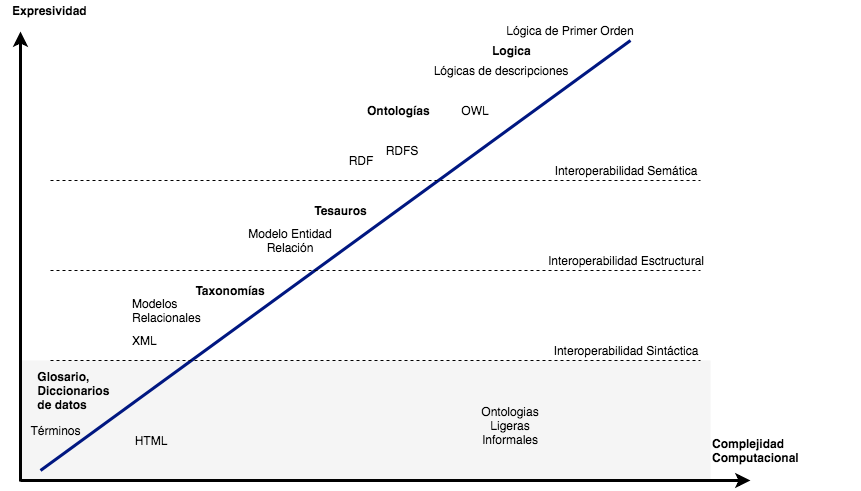
\includegraphics[width=150mm]{figuras/Diagramas-ComplejidadOntologica}
    \caption{Expresividad vs Complejidad. Adaptación de \cite{Giunchiglia2009LightweightO} \cite{Obrst}}
    \label{img:expresividad complejidad }
    \end{figure}



\section{RDF y RDFS (RDF)}

Marco de Descripción de Recursos, RDF por sus siglas \textit{Resource Description Framework}  \cite{rdf}, es un framework para representar información en la Web Semántica. El lenguaje RDF forma parte de la W3C's \textit{Semantic Web Activity} y es recomendado por la W3C \cite{Semantic20:online}. El modelo de datos RDF está diseñado para que sea procesable por computadoras. 

RDF nos permite representar modelos de datos basados en grafos, los cuales son representados en triplas. Las triplas RDF contienen tres componentes:

\begin{itemize}
  \item El sujeto, que puede ser una referencia tipo URI o un \textit{Blank Node}
  \item El predicado, que es una referencia tipo URI
  \item El objeto que puede ser una referencia tipo URI, un literal o un \textit{Blank Node}
\end{itemize}



En la Figura \ref{img:componentes rdf } se expone un grafo de ejemplo en el cual se visualizan estos tres componentes.

    \begin{figure}[ht!]
    \centering
    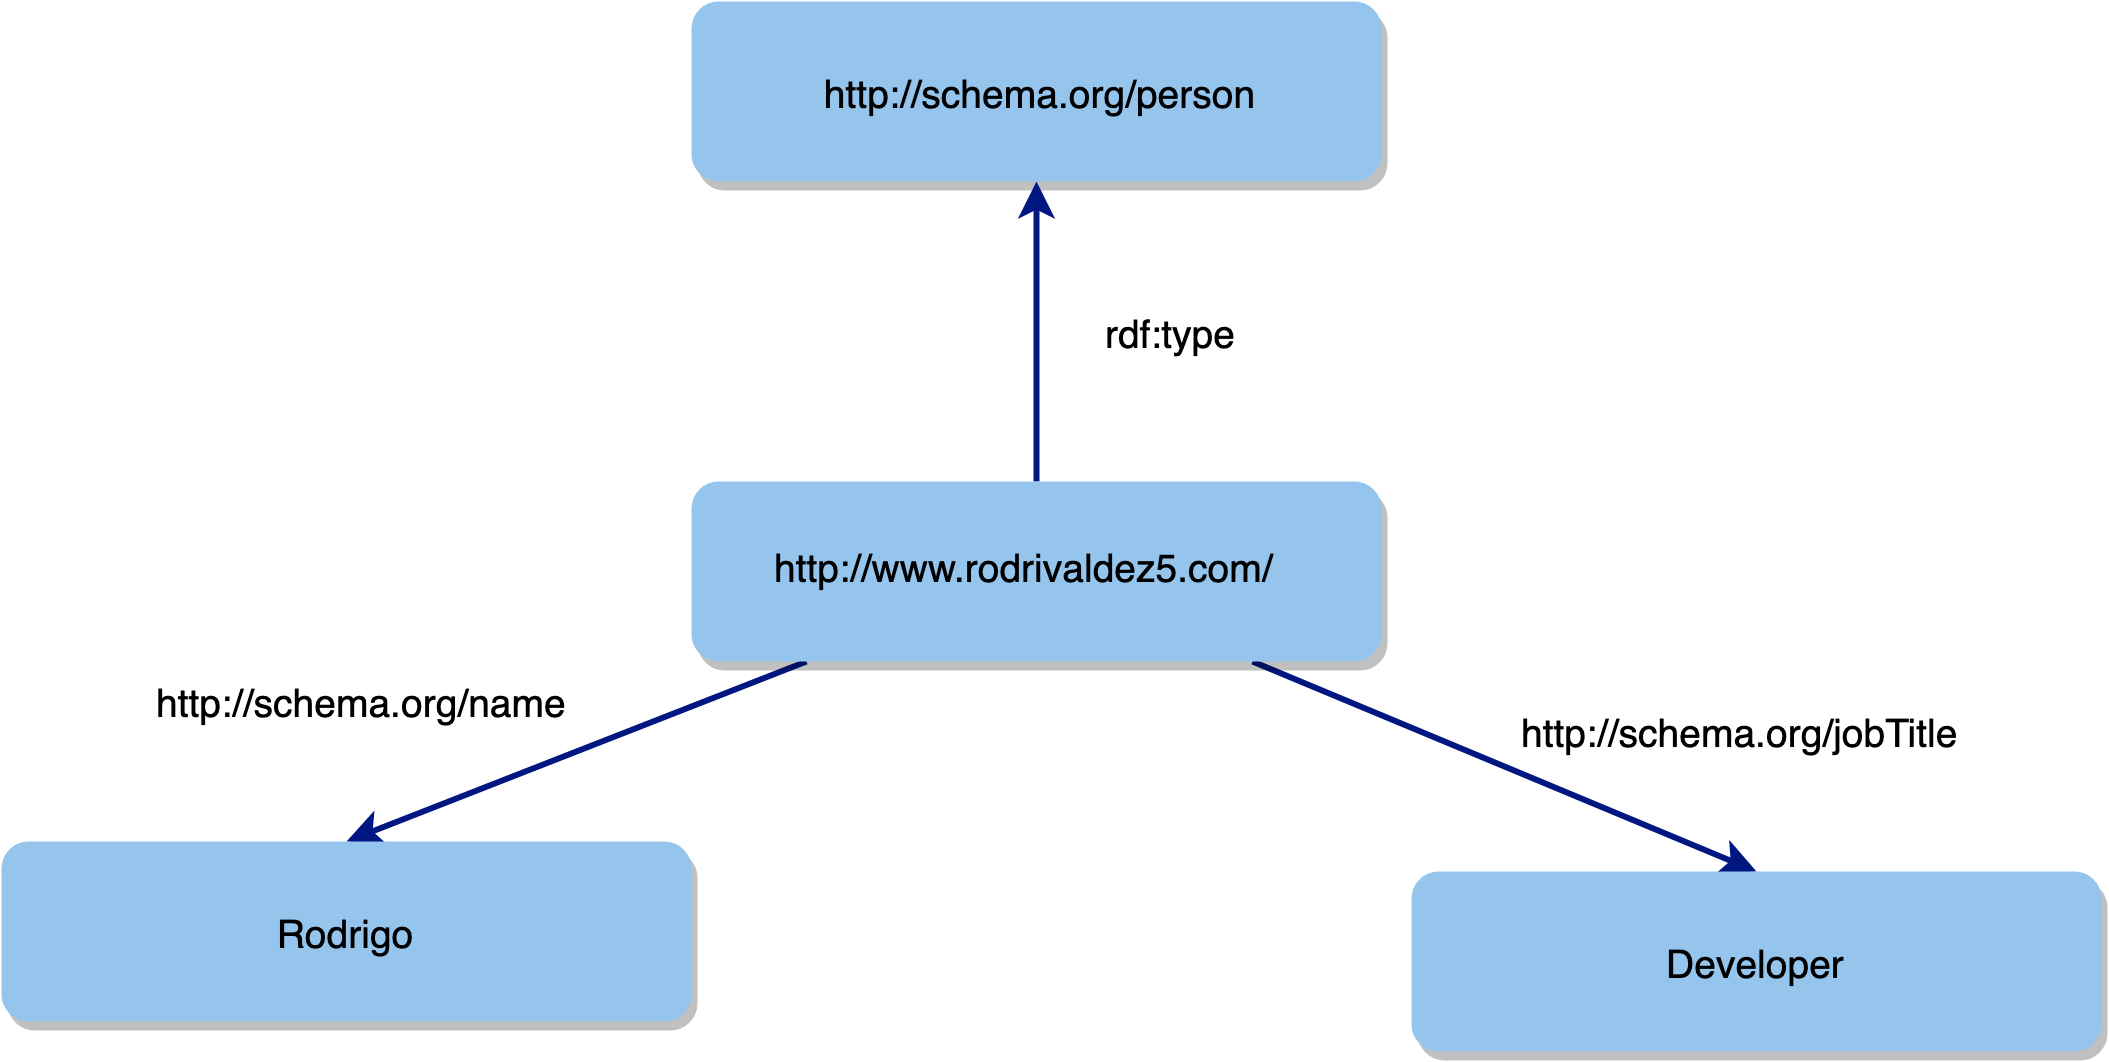
\includegraphics[width=150mm]{figuras/Diagramas-RDFGraph}
    \caption{Componentes RDF}
    \label{img:componentes rdf }
    \end{figure}
    
El sujeto es la fuente de la arista y debe ser un recurso. En RDF, un recurso puede ser cualquier cosa que sea identificable de forma única a través de un URI. Comúnmente este identificador es un URL, que es un caso especial de URI. Sin embargo, los URI son más generales que las URL. En particular, no es requerimiento que un URI se pueda utilizar para localizar un documento en Internet. El objeto de una sentencia es el objetivo de la arista. Al igual que el sujeto, puede ser un recurso identificado por un URI, pero alternativamente puede ser un valor literal como una cadena o un número. Los predicados de una sentencia determinan qué tipo de relación se mantiene entre el sujeto y el objeto. También es identificado por un URI.

Un identificador uniforme de recursos \footnote{https://www.w3.org/wiki/URI} (URI por sus siglas inglés \textit{Uniform Resource Identifier}) es una cadena de caracteres que identifica inequívocamente un recurso en particular. 

Todos los literales tienen una forma léxica que es una cadena \textit{Unicode}. Un literal en un grafo RDF puede presentarse de dos formas:
\begin{itemize}
    \item Los literales simples tienen una forma léxica y, opcionalmente, una etiqueta de idioma normalizada a minúscula. Ej.: “Hola mundo”@es.
    \item Los literales tipados que tienen una forma léxica y una URI de tipo de datos que es una referencia de URI RDF. Ej.: “Hola mundo”\textit{xsd:string}.
\end{itemize}

Un \textit{Blank Node} es un nodo en un documento RDF que representa un recurso para el que no se proporciona un URI o literal y también es llamado recurso anónimo.

RDF es simplemente un representación sictáctica de datos y no provee significado semántico de los mismos. RDF Schema (RDFS) en cambio es una extensión de RDF que nos permite definir un vocabulario para el uso en modelos de datos RDF, permite definir tipo de clases de un recurso y propiedades que un recurso puede tener, esto a través de un vocabulario que incluye\textit{ rdfs:Class, rdf:Property , rdfs:subClassOf, rdfs:subPropertyOf, rdfs:domain, rdfs:range} y otras propiedades de documentación como son \textit{rdfs:label y rdfs:comment}.

La sintaxis de RDF puede escribirse en distintos formatos de serialización: \textit{RDF/XML \footnote{https://www.w3.org/TR/2004/NOTE-owl-parsing-20040121/}, Turtle\footnote{https://www.w3.org/TR/turtle/}, N-Triples \footnote{https://www.w3.org/TR/n-triples/}, N-Quads \footnote{https://www.w3.org/TR/n-quads/} y JSON-LD\footnote{https://json-ld.org/spec/latest/json-ld-rdf/}}.

En el Cuadro \ref{lst:n-quads} se muestra un ejemplo de triplas en formato RDF/N-Quads. \hfill \break

\lstset{language=XML}
    
\noindent\begin{minipage}{\textwidth}
\begin{lstlisting}[captionpos=b, caption=Ejemplo en RDF/N-Quads, label=lst:n-quads,  numbers=left,  numberstyle=\tiny\color{mygray},frame=single]
<http://rodrivaldez5.com/> <http://www.w3.org/2000/01/rdf-schema#type> <http://schema.org/person> .  
<http://www.rodrivaldez5.com/> <http://schema.org/name>"Rodrigo Valdez" .
<http://www.rodrivaldez5.com/> <http://schema.org/telephone>"0981530572" .
<http://www.rodrivaldez5.com/> <http://schema.org/jobTitle>"Developer" .
<http://www.rodrivaldez5.com/> <http://schema.org/image> <http://www.rodrivaldez5.com/images/rodri.png> .
\end{lstlisting}
\end{minipage}

En linea 1, <http://www.rodrivaldez5.com/> es el sujeto, <http://schema.org/image>  es el predicado y <http://www.rodrivaldez5.com/images/rodri.png>  es el objeto, donde el objeto en este caso es una URI. En la línea 2 se puede ver que el objeto se trata de un dato literal de tipo String.  A continuación se presenta JSON-LD, una forma de representación de datos compatible con RDF.

\subsection{Serialización JSON-LD}

JSON, por sus siglas en inglés \textit{JavaScript Object Notation} es un formato de texto utilizado para la representación e intercambio de datos en la web. JSON-LD \cite{JSONLDSy39:online}, donde LD proviene de \textit{Linked Data}, es una extensión de JSON cuya idea es lograr el enlace de datos y agregar una capa de semántica a la web. JSON-LD define un mecanismo para mapear los términos JSON (propiedad y valor) a URIs que poseen información semántica acerca del término. 

Todo objeto JSON-LD es también un objeto JSON. JSON-LD es compatible con RDF ya que se puede representar en triplas, en este caso el nombre de la propiedad (JSON) corresponde al predicado (RDF), el sujeto (RDF) corresponde al objeto (JSON) y el valor de la propiedad (JSON) corresponde al objeto (RDF).

A continuación se plantea un ejemplo de transformación de un documento JSON a JSON-LD 

En el Cuadro \ref{lst:json} se muestra un ejemplo de documento JSON y en el Cuadro \ref{lst:json-ld} se muestra su transformación a JSON-LD.  
\newline

\lstset{language=json}  

\noindent\begin{minipage}{\textwidth}
\begin{lstlisting}[captionpos=b, caption=Ejemplo de un documento JSON, label=lst:json,  numbers=left,  numberstyle=\tiny\color{mygray},frame=single]
{
  "id": "http://www.rodrivaldez5.com/",
  "name": "Rodrigo Valdez",
  "telephone": "0981530572",
  "jobTitle": "Developer",
  "image": "http://www.rodrivaldez5.com/images/rodri.png"
}
\end{lstlisting}
\end{minipage}

\noindent\begin{minipage}{\textwidth}
\begin{lstlisting}[captionpos=b, caption=Ejemplo de un documento JSON-LD, label=lst:json-ld,  numbers=left,  numberstyle=\tiny\color{mygray},frame=single]
{
  "@id": "http://www.rodrivaldez5.com/",
  "@type": "http://schema.org/person",
  "http://schema.org/name": "Rodrigo Valdez",
  "http://schema.org/telephone" : "0981530572",
  "http://schema.org/jobTitle": "Developer",
  "http://schema.org/image":   {"@id":  "http://www.rodrivaldez5.com/images/rodri.png"} 
}
\end{lstlisting}
\end{minipage}
De aquí se puede observar que el principal cambio radica en los nombres de las propiedades, las cuales ahora son URIs válidos, el resultado es equivalente a las triplas RDF del Cuadro \ref{lst:n-quads}

Además JSON-LD permite crear un contexto que contiene el mapeamiento entre el nombre de la propiedad y la URI, dando como resultado el objeto JSON-LD del Cuadro \ref{lst:json-ld-contexto}. \hfill \break

\noindent\begin{minipage}{\textwidth}
\begin{lstlisting}[captionpos=b, caption=Ejemplo de un documento JSON-LD con Contexto, label=lst:json-ld-contexto,  numbers=left,  numberstyle=\tiny\color{mygray},frame=single]
{
  "@context": {
    "name": "http://schema.org/name",  
    "joTitle": "http://schema.org/jobTitle",  
    "telephone": "http://schema.org/telephone",  
    "image": {
      "@id": "http://schema.org/image",  
      "@type": "@id"  
    },
  
  },
  "@id": "http://www.rodrivaldez5.com/",
  "@type": "http://schema.org/person",
  "image": "http://www.rodrivaldez5.com/images/rodri.png",
  "jobTitle": "Developer",
  "name": "Rodrigo Valdez",
  "telephone": "0981530572"
}
\end{lstlisting}
\end{minipage}
El contexto también puede definirse en otro documento diferente y solamente haciendo referencia a éste, quedando el JSON final como se muestra en el Cuadro \ref{lst:json-ld-contexto-referencia}

\noindent\begin{minipage}{\textwidth}
\begin{lstlisting}[captionpos=b, caption=Ejemplo de un documento JSON-LD con Contexto referenciado, label=lst:json-ld-contexto-referencia,  numbers=left,  numberstyle=\tiny\color{mygray},frame=single]
{
  "@context": "http://schema.org/",
  "@id": "http://www.rodrivaldez5.com/",
  "http://schema.org/name": "Rodrigo Valdez",
  "http://schema.org/telephone" : "0981530572",
  "http://schema.org/jobTitle": "Developer",
  "http://schema.org/image":   {"@id": "http://www.rodrivaldez5.com/images/rodri.png"} 
}
\end{lstlisting}
\end{minipage}
El formato JSON es ampliamente utilizado y preferido por los desarrolladores en la web, en comparación con el formato de representación RDF. En la Tabla \ref{prefencia-uso} se muestra la preferencia de uso entre la serialización RDF y JSON-LD en algunas categorías de aplicaciones \cite{rdfjson}.

\begin{table}[!htb]
\footnotesize
\centering
\caption{Preferencias de uso de serialización RDF y JSON-LD \cite{RDFANDJS70:online}}
\label{prefencia-uso}
\resizebox{15cm}{!} {
\begin{tabular}{|l|l|l|}
\hline
 \thead{Categoría de Aplicación} & \thead{RDF o JSON-LD} & \thead{Comentarios}\\\hline
\multicolumn{1}{|m{5cm}|}{Aplicación Web API} & JSON-LD & \multicolumn{1}{m{5cm}|}{La sintaxis está diseñada para integrar fácilmente en sistemas desplegados que ya usan JSON, y proporciona un camino de actualización sin problemas de JSON a JSON-LD}\\\hline
\multicolumn{1}{|m{5cm}|}{Aplicaciones de UI basadas en navegador} & JSON-LD & \multicolumn{1}{m{5cm}|}{La gran cantidad de parsers basados en JSON. Javascript es el lenguaje del navegador}\\\hline
\multicolumn{1}{|m{5cm}|}{Aplicaciones basadas en Inferencia, Razonamiento} & RDF & 
\multicolumn{1}{m{5cm}|}{Gran soporte para razonadores y almacenes de tripletas escalables}\\\hline
\multicolumn{1}{|m{5cm}|}{Herramientas de consultas Expresivas} & RDF & \multicolumn{1}{m{5cm}|}{El estado avanzado de SPARQL 1.1 ayuda a escribir consultas potentes y expresivas}\\ \hline
\end{tabular}
}
\end{table}



\section{\textit{Web Ontology Language }(OWL)}
OWL es un estándar internacional para codificar e intercambiar ontologías y es diseñado para soportar la Web Semántica.

Es el lenguaje de representación de conocimientos recomendado por la W3C y es una extensión de RDFS, dándole mayor expresividad a través de operaciones booleanas (intersección, unión, complemento), restricciones de cardinalidad, cuantificación existencial, etc. El mismo está basado en lenguajes de representación de conocimientos llamados Lógica de Descripciones (DL, por sus siglas en inglés \textit{Description Logic}). DL es un lenguaje formal usado para construir ontologías y permite declarar conocimiento de un dominio específico e incluir reglas de razonamiento para poder procesarlo \cite{kalibatiene2011survey}.

Al estar basado en DL, OWL nos trae consigo las siguientes ventajas
\begin{itemize}
    \item Expresividad: La Lógica de Descripciones nos permite tener expresiones complejas de los conceptos a modelar.
    \item Razonador Automático: La Lógica de Descripciones está basado en lógica formal, eso nos permite desarrollar razonadores capaces de verificar la consistencia de la ontológica e inferir nuevo conocimiento.
\end{itemize}

OWL posee tres sub lenguajes: OWL Lite, OWL DL y OWL Full. Todos permiten describir clases, propiedades e instancias pero difieren uno de otro en el nivel de especificación requerido. OWL Lite está diseñado para usuarios cuyas necesidades de modelado sean simples. OWL DL es lo más cercano a una DL expresiva manteniendo la completitud computacional, esto significa que la ontología es procesable computacionalmente. OWL Full posee mayor expresividad sacrificando la completitud computacional de la ontología. En la Figura \ref{img:subclases owl} se muestra la relación entre los tres sublenguajes.

\begin{figure}[h!]
    \centering
    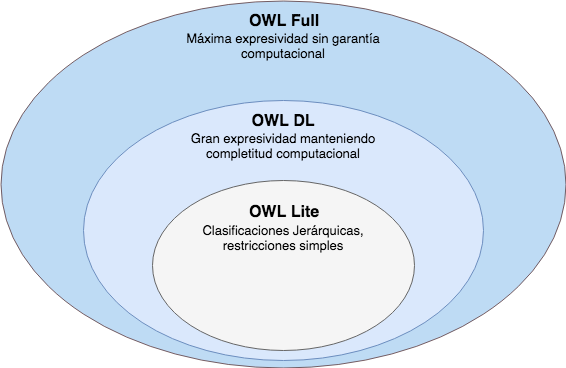
\includegraphics[width=150mm]{figuras/Diagramas-OwlSubClasses.png}
    \caption{Subclases OWL. \cite{owllevels}}
    \label{img:subclases owl}
    \end{figure}

OWL DL posee todas las características de OWL Lite más sus propias complejidades. OWL Full posee las mismas características de OWL DL agregando otras que resultan en mayor complejidad.

\section{Metodologías para el desarrollo de Ontologías}

En este apartado se dará un resumen de las metodologías más utilizadas para la creación de una ontología; Ontology Development 101, OntoKnowledge , Methontology, y NeOn. Luego se realizará un análisis y elección según los requerimientos de este trabajo.

\subsection{Ontology Development 101}

Esta metodología describe una serie de pasos y recomendaciones a la hora de crear una ontología. 

Se describen a continuación los pasos:
\begin{description}
\item[Paso 1:] Determinar el dominio y alcance de la ontología.
\item[Paso 2:] Considerar la reutilización de ontologías.
\item[Paso 3:] Enumerar términos importantes de la ontología.
\item[Paso 4:] Definir las clases y las jerarquías de las clases.
\item[Paso 5:] Definir las propiedades de las clases.
\item[Paso 6:] Definir las características de cada clase y propiedad.
\item[Paso 7:] Crear instancias.
\end{description}

Además la guía propone algunas buenas prácticas de desarrollo de ontologías relacionadas a la definición de clases como la correcta creación de jerarquías, herencias múltiples,  cuándo crear una clase o una propiedad, cuando es una instancia o una clase, etc. También algunos delineamientos sobre las propiedades como valores por defecto, cardinalidad, etc. Por último, una serie de convenciones de nombres dentro de la ontología. La metodología no tiene en cuenta el proceso de especificación ni el mantenimiento de la ontología.

\subsection{OntoKnowledge} 

Ontoknowledge propone crear ontologías teniendo en cuenta su uso posterior en sistemas de administración de conocimiento, por tanto las ontologías creadas son dependientes de la aplicación. La metodología incluye la identificación de metas a ser logradas a través de herramientas de control basadas en los escenarios de usos.

El proceso que propone la metodología se puede resumir en los siguientes pasos:

\textbf{Estudio de Factibilidad.} Esta debe ser aplicada a toda la aplicación y debe llevarse a cabo antes del desarrollo de la ontología. Aquí se identifica el problema y las áreas de oportunidades, se selecciona la mejor área de enfoque para la solución.

\textbf{Patada Inicial.} El resultado de este proceso es el Documento de Especificación de Requerimientos de la Ontología (ORSD). Se describen las metas y el dominio de la ontología, líneas de diseño (convenciones de nombres), lista de recursos disponibles (libros, revistas, documentación, etc), potenciales usuarios y casos de uso, así como las aplicaciones que utilizarán la ontología. Para esto se propone crear una lista de preguntas de competencia las cuales debe satisfacer la ontología creada. Los conceptos y relaciones más importantes son identificados en un nivel informal. También se debe de buscar ontologías para su potencial reuso, la metodología no provee un delineamiento para identificar dichas ontologías.

\textbf{Refinamiento.} Aquí se construye una ontología sólida orientada a la aplicación acorde al proceso de especificación. Este proceso se divide en dos actividades:

\begin{description}
\item[Actividad 1:] Extracción del conocimiento del los expertos del dominio. Los axiomas de la ontología son definidos y modelados por los expertos del dominio. La metodología propone el uso de una representación intermedia para modelar el conocimiento.
\item[Actividad 2:] Formalización de la ontología. La ontología es implementada en un lenguaje ontológico, el lenguaje es seleccionado según los requerimientos del uso de la ontología.
\end{description}

\textbf{Evaluación.} Este paso sirve para probar la usabilidad de la ontología desarrollada dentro del entorno para la cual fue desarrollada. En este proceso se verifica que se puedan responder las preguntas de competencia y que se satisfagan los requerimientos, además se prueba la ontología en el entorno de software para el cual se desarrolló.

\textbf{Mantenimiento.} En esta etapa es importante recalcar quién es el responsable de mantener la ontología y cómo se debe hacerlo.

La metodología propone un ciclo de vida incremental y cíclico como se muestra en la Figura \ref{img:ontoknowledge}.

\begin{figure}[h!]
    \centering
    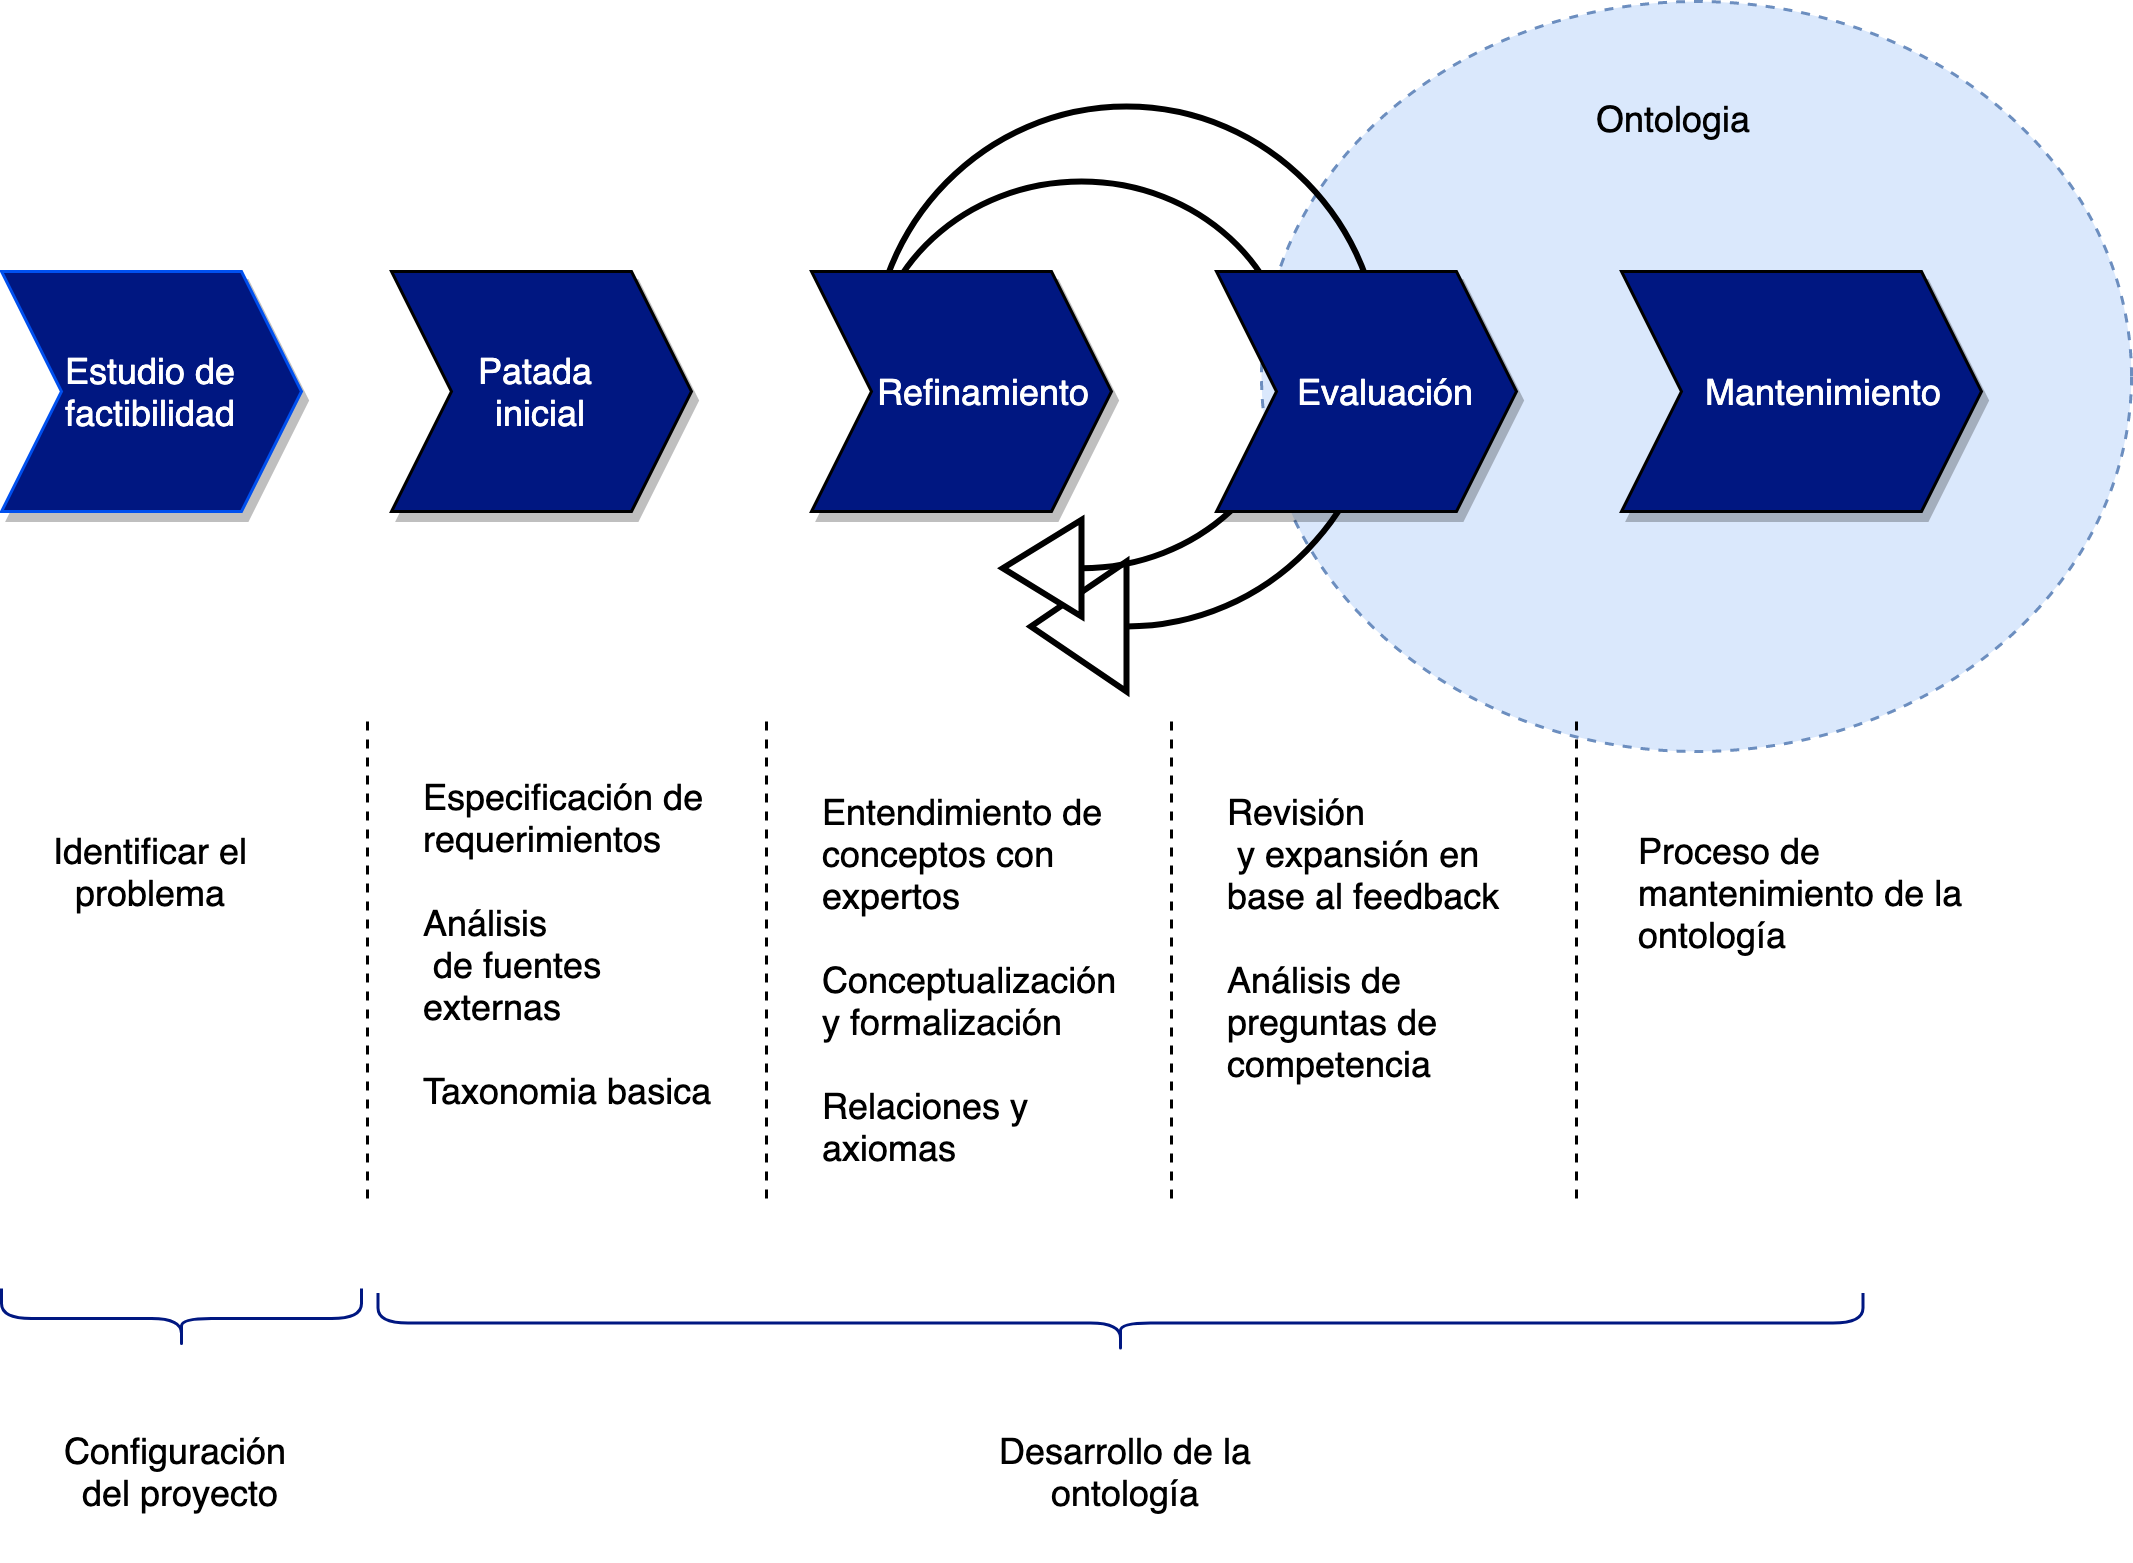
\includegraphics[width=150mm]{figuras/Diagramas-OntoKnowledgeProcess}
    \caption{Ciclo de vida de OntoKnowledge}
    \label{img:ontoknowledge}
    \end{figure}

\subsection{Methontology}

Esta metodología incluye la identificación del proceso del desarrollo de una ontología, que consiste en una serie de actividades, el ciclo de vida basado en el refinamiento de un prototipo y técnicas para llevar a cabo cada actividad durante el mantenimiento, el desarrollo y el soporte de las actividades. Todas las actividades están basadas en el proceso de desarrollo de software y las utilizadas en metodologías de ingeniería de conocimiento.

En la Figura \ref{img:methontology} se puede ver los estados de todo el ciclo de vida de la ontología.

\begin{figure}[h!]
    \centering
    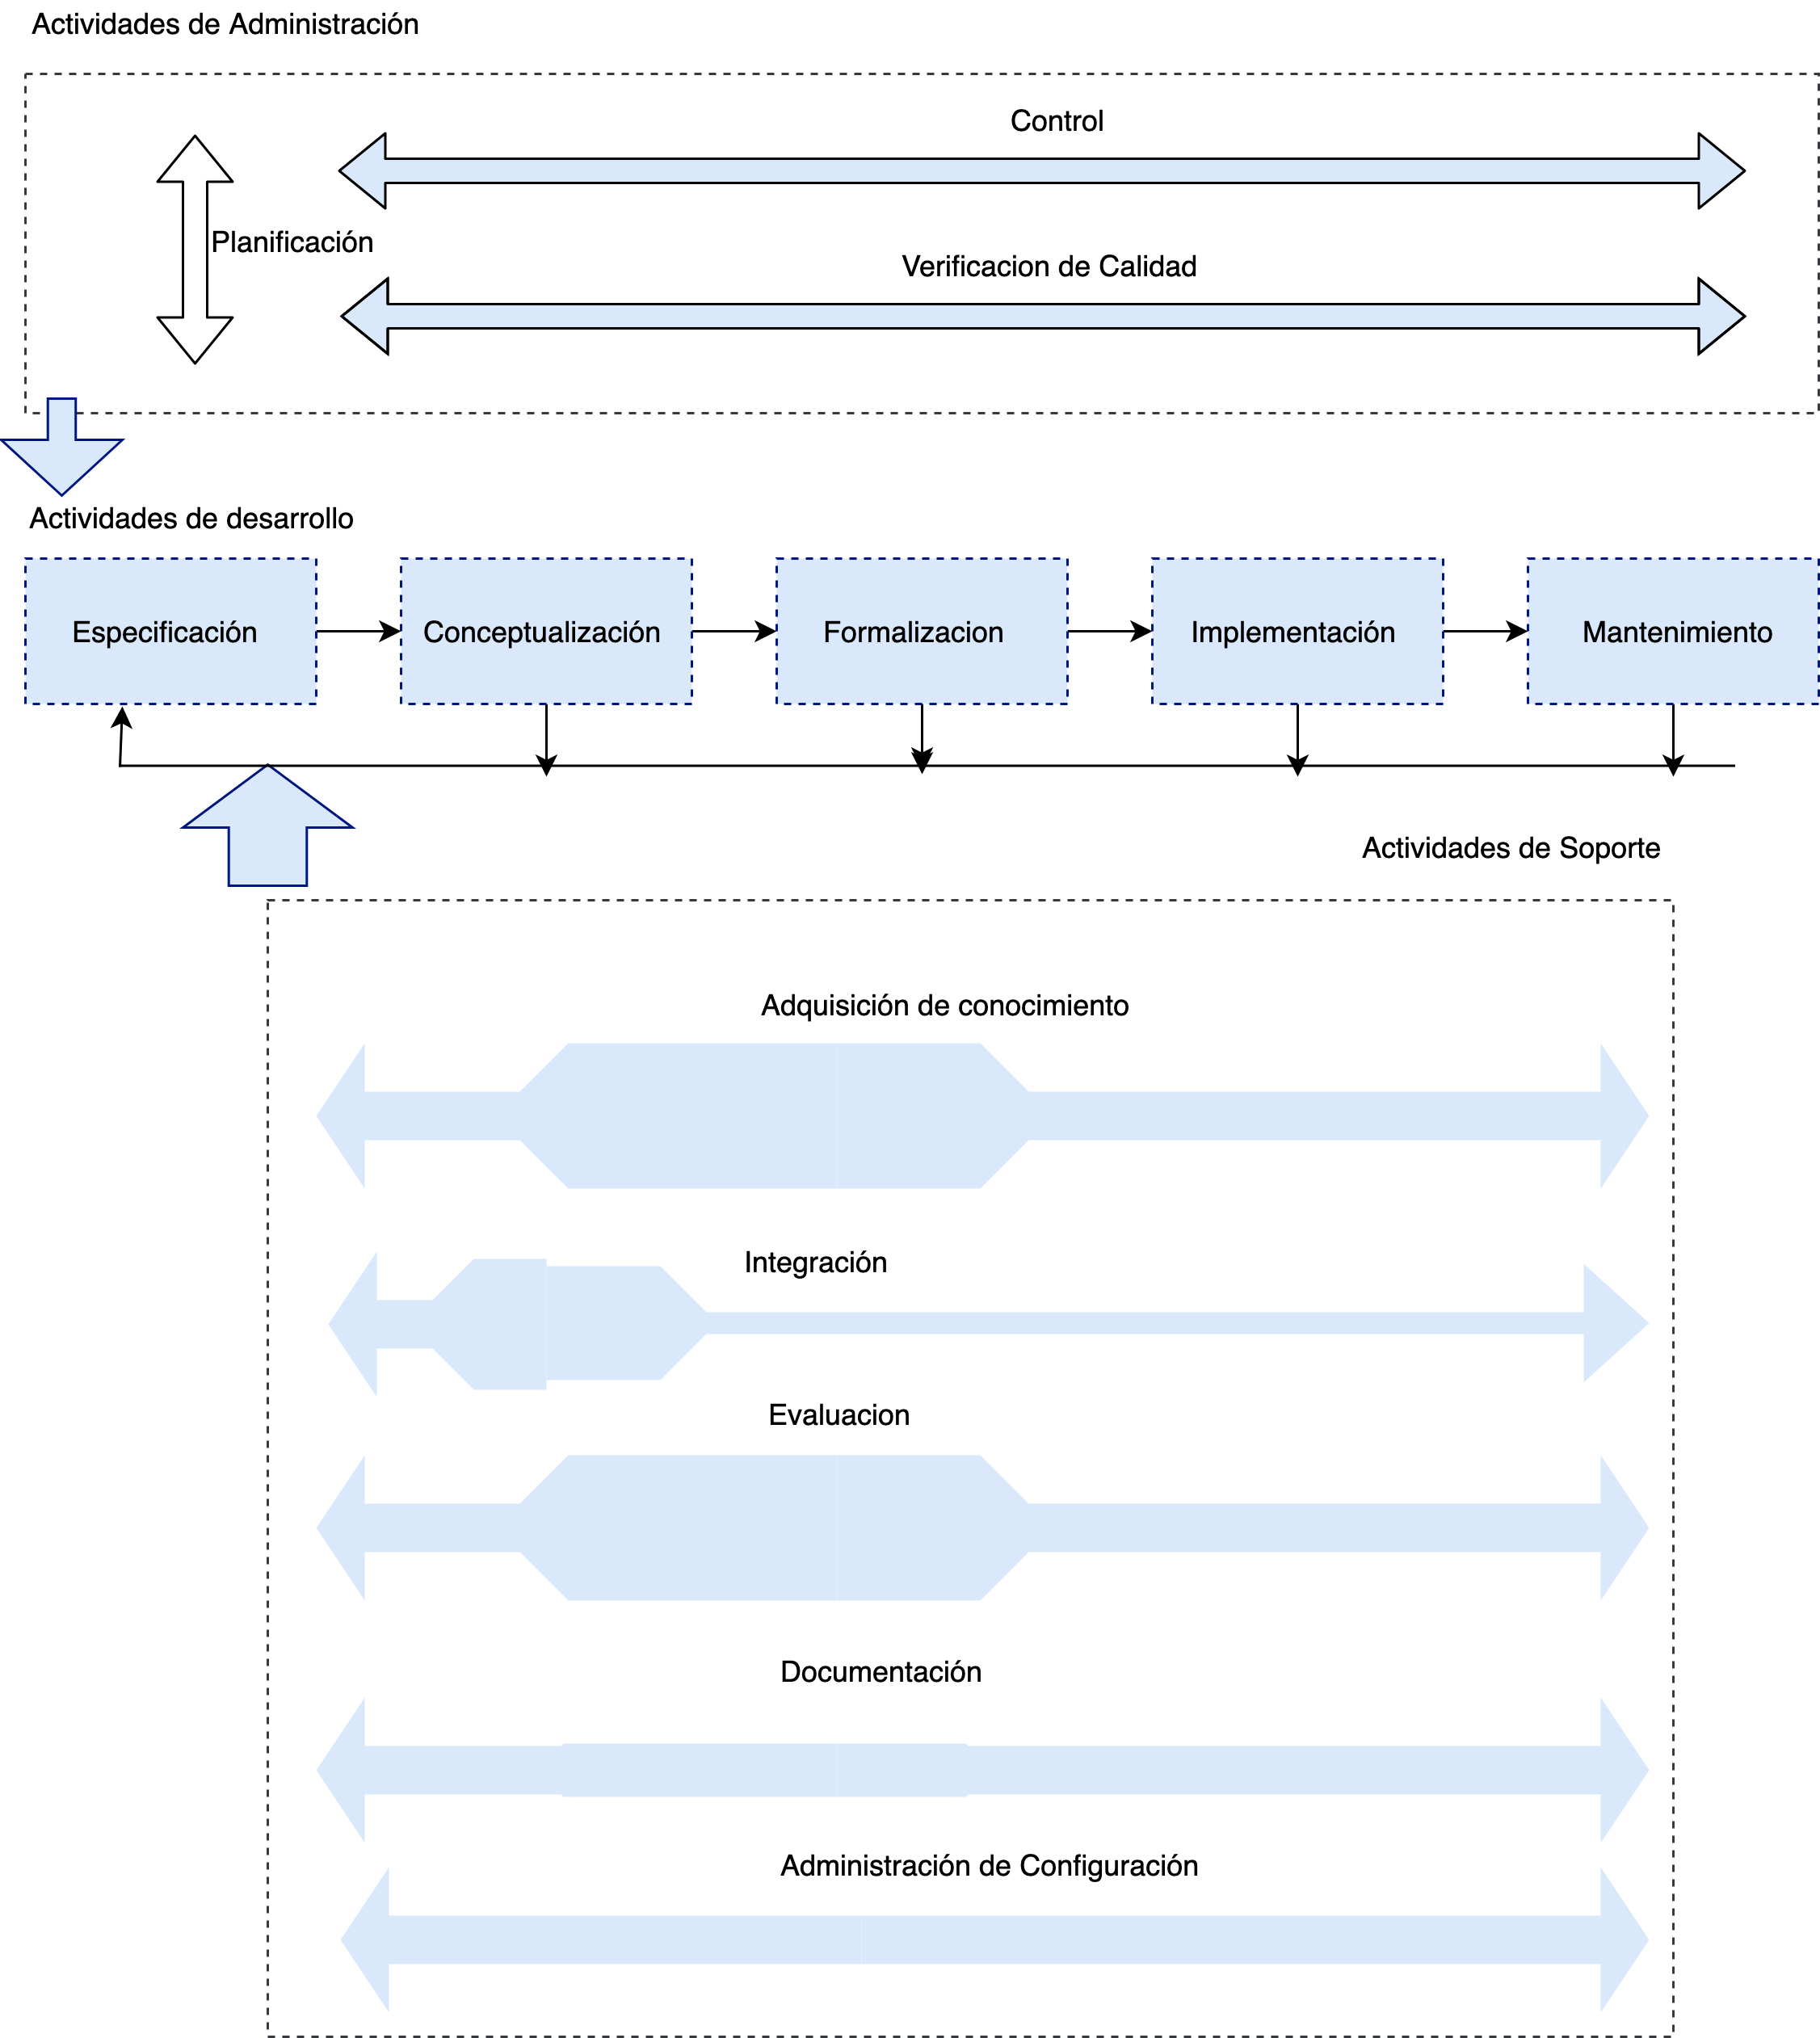
\includegraphics[width=150mm]{figuras/Diagramas-MethontologyProcess}
    \caption{Ciclo de vida de Methontology}
    \label{img:methontology}
    \end{figure}
    
    
La metodología propone un ciclo de vida basado en prototipos que permite agregar, cambiar y remover términos en cada prototipo. Para cada prototipo, se propone comenzar con la planificación para identificar las tareas, tiempos y recursos necesarios. Luego, comienza la actividad de especificación, con ella comienzan las actividades de gestión (Control y Calidad) y procesos de soporte (Adquisición de conocimiento, integración, evaluación, documentación y gestión de la configuración), todo esto ejecutado en forma paralela a las actividades de desarrollo (especificación, conceptualización, implementación y mantenimiento) durante todo el ciclo de vida de la tecnología \cite{fernandez1997methontology}.
 
A continuación se describen algunas de las principales actividades:

\begin{enumerate}
\item \textbf{Especificación:} Especificar el propósito de la ontologías, esto incluye usuarios, contexto, nivel de formalidad esperado y granularidad. El resultado de esta fase es un documento de especificación de la ontología en lenguaje natural.
\item \textbf{Adquisición} de conocimiento: Esto ocurre en paralelo a las demás fases, pero específicamente en la parte de especificación. Se consultan libros, manuales, tablas, otras ontologías y expertos para adquirir conocimientos sobre el área a modelar.
\item \textbf{Conceptualización:} Se identifican los términos según sean conceptos, instancias, relaciones o propiedades para crear un modelo conceptual del dominio.
\item \textbf{Integración:} En esta fase se considera el reuso de términos de otras ontologías para no volver a definir y ahorrar trabajo.
\item \textbf{Implementación:} La ontología es representada formalmente en un lenguaje tipo OWL o RDFS.
\item \textbf{Evaluación:} Significa hacer un juzgamiento técnico de la ontología creada, el entorno de desarrollo y la documentación de la misma. La evaluación está compuesta por la verificación y la validación.
\item \textbf{Documentación:} El cual consiste en todos los documentos producidos durante el desarrollo de la ontología que va desde el mismo código de la ontología hasta artículos científicos de la misma.
\end{enumerate}


\subsection{NeOn}
Esta metodología incluye métodos, técnicas y herramientas para llevar a cabo actividades para el proceso de desarrollo de una red ontológica. Está enfocada en la especificación de los requerimientos, la planificación y el reuso de recursos ontológicos y no-ontológicos \cite{suarez2010neon}.

La metodología presenta los siguientes componentes:
\begin{itemize}
    \item Un glosario: Identifica y define los procesos y actividades que pueden estar dentro de el desarrollo de una ontología. En la Figura \ref{img:neon actividades} se muestra la lista de procesos y actividades divididas según la fase de desarrollo.
    \item Nueve escenarios para el desarrollo de ontologías. Se identificaron nueve escenarios flexibles para el desarrollo de ontologías, donde cada escenario está compuesto de diferentes procesos y actividades. En la Figura \ref{img:neon ciclo de vida} se distinguen las relaciones entre las actividades y los escenarios donde las fechas dirigidas con círculos numerados asociados representan los diferentes escenarios. 
    \item Una serie de guías metodológicas para procesos y actividades como el reuso de recursos ontológicos y no-ontológicos, la especificación de los requerimientos, la planificación, etc. Los procesos y actividades están representados en la Figura \ref{img:neon ciclo de vida} con cajas y círculos de color.
\end{itemize}

A continuación se presenta el glosario de términos:
\begin{figure}[h!]
    \centering
    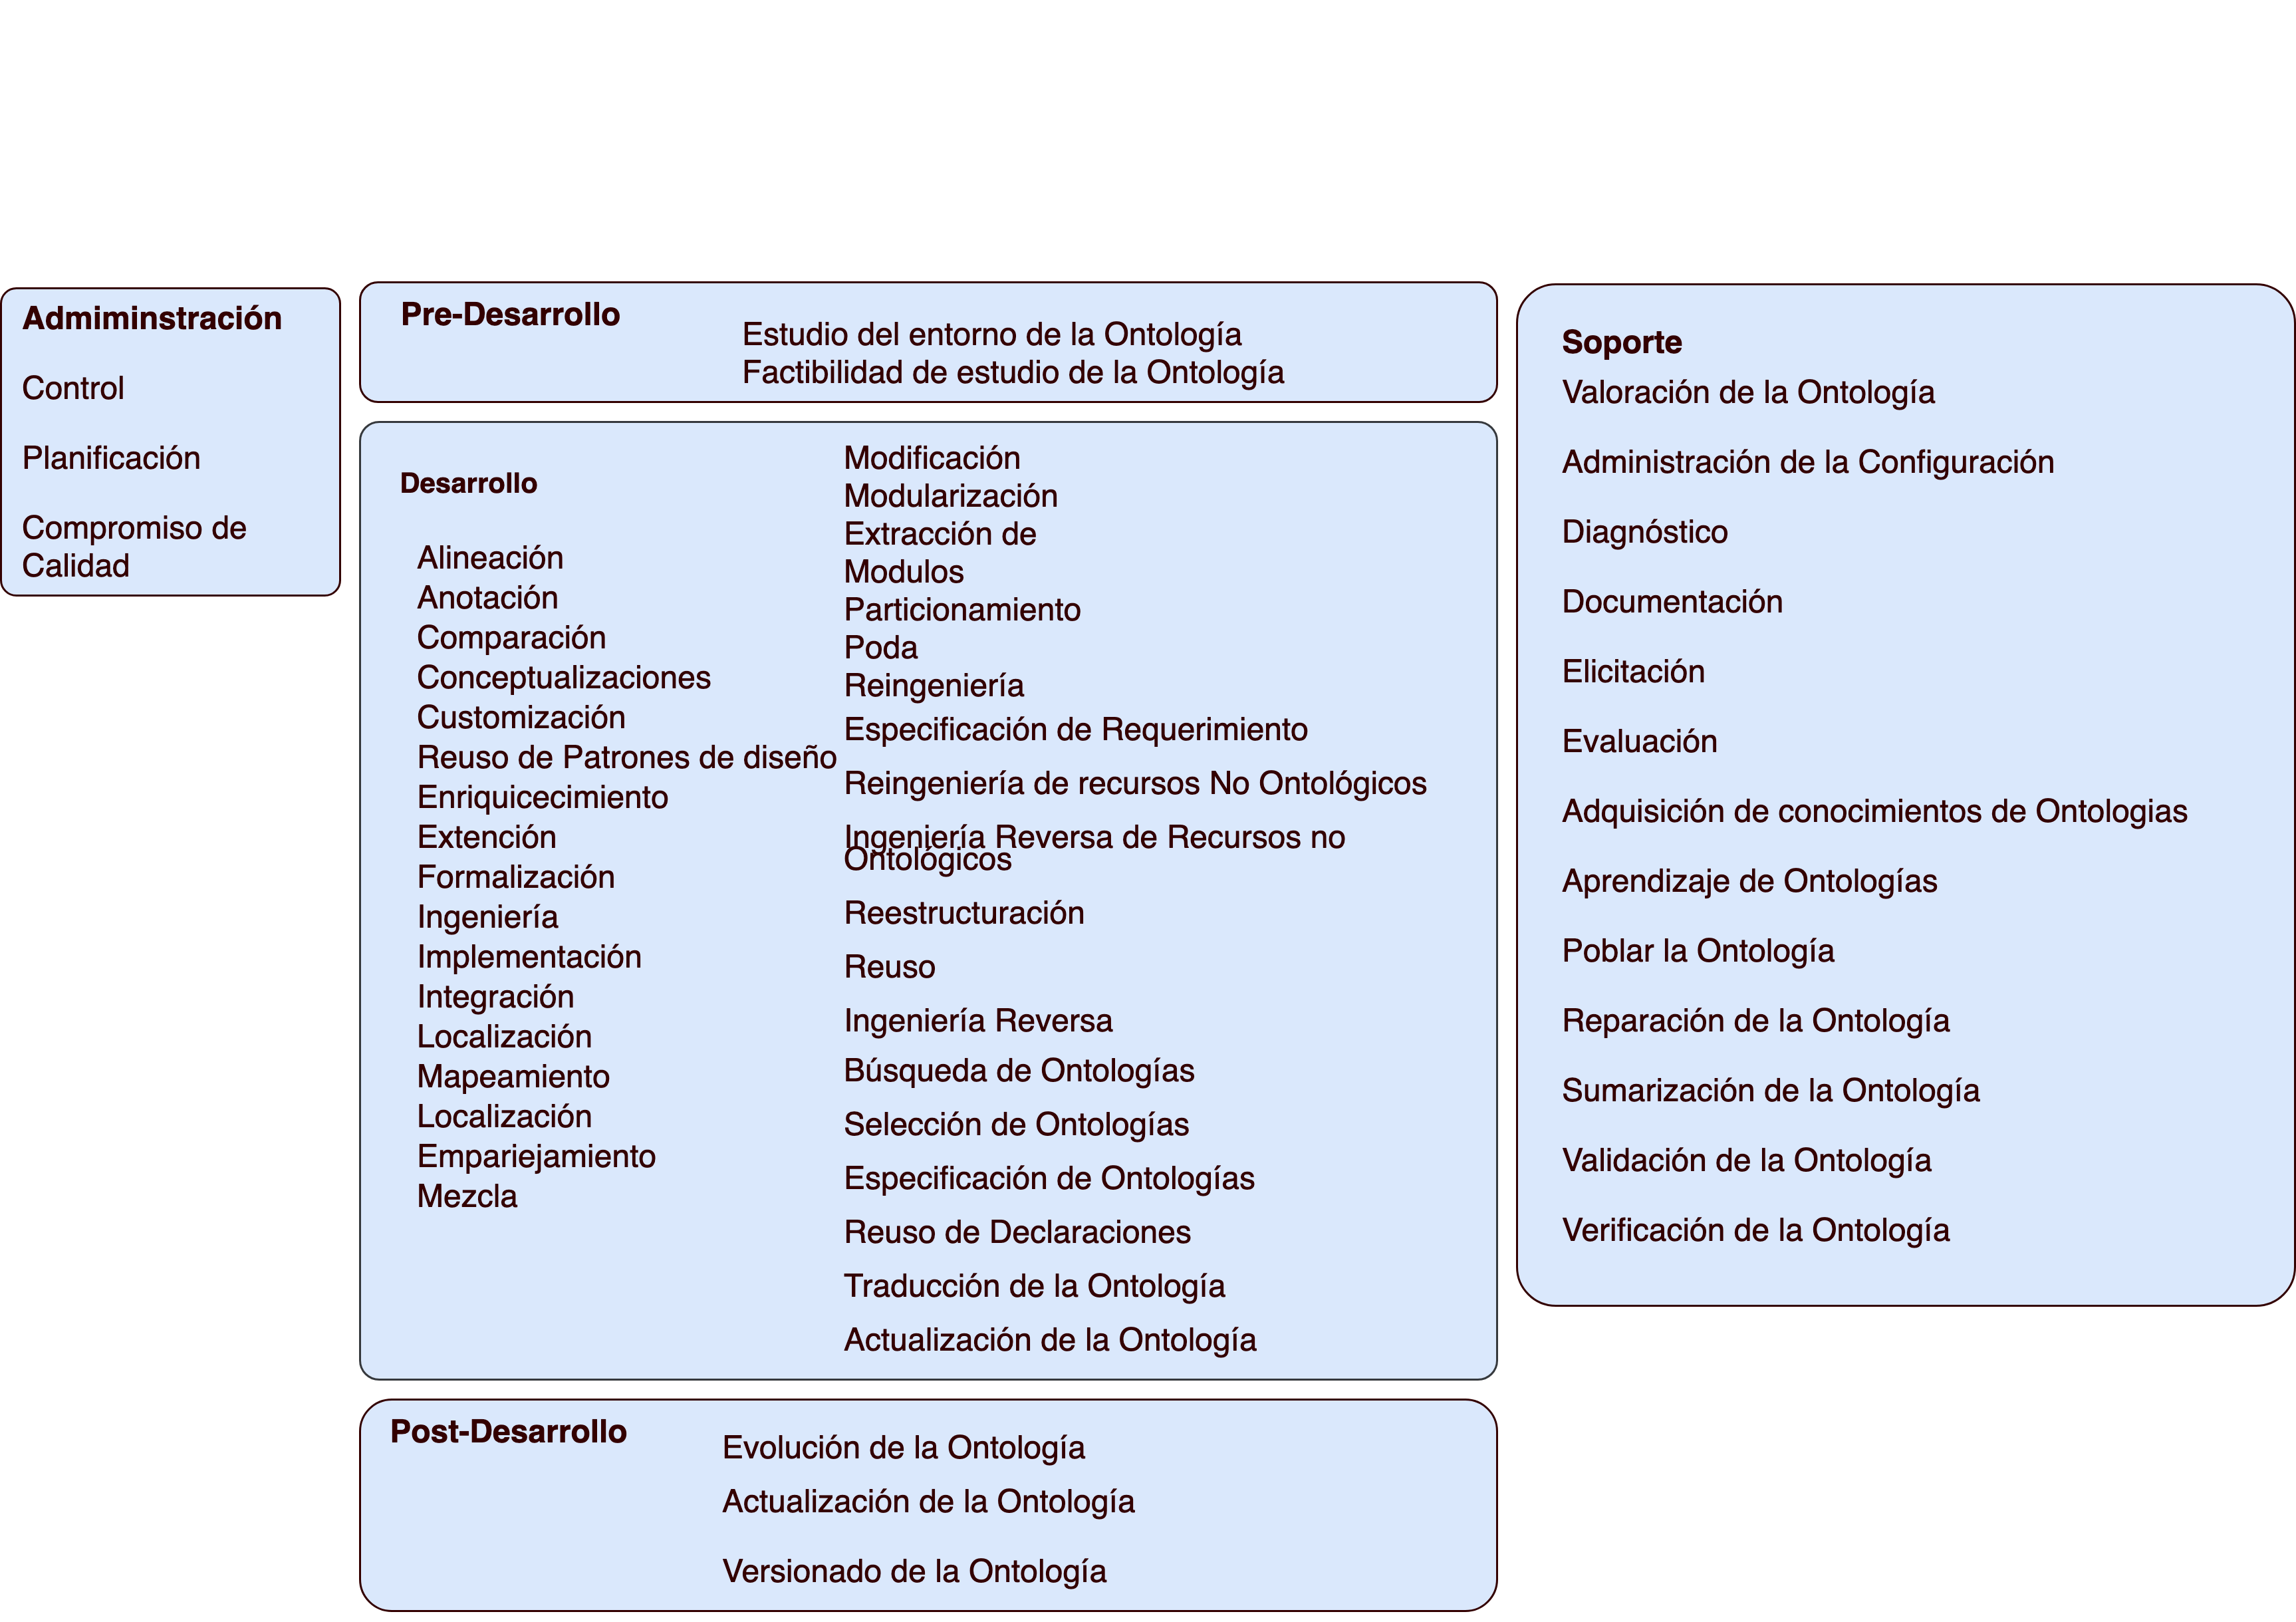
\includegraphics[width=150mm]{figuras/Diagramas-NeonActivities}
    \caption{Actividades de NeOn}
    \label{img:neon actividades}
    \end{figure}


A continuación se presentan los nueve escenarios que propone NeOn.

\begin{description}
    \item[Escenario 1] El escenario va desde la especificación hasta la implementación. La ontología es desarrollada desde el principio, esto significa sin utilizar ninguna base de conocimiento ya construida.
    \item[Escenario 2] Reuso y Reingeniería de recursos no-ontológicos. Este escenario cubre el caso donde los desarrolladores analizan recursos no-ontológicos, y deciden según los requerimientos, qué recurso no-ontológico se puede reutilizar para construir esta ontología. Este escenario también realiza una reingeniería del recurso seleccionado.
    \item[Escenario 3] Reuso de recursos ontológicos. En este escenario los desarrolladores reusan recursos ontológicos, esto se puede hacer de tres maneras: reuso total, reuso de módulos y/o reuso de sentencias.
    \item[Escenario 4] Reuso y reingeniería de recursos ontológicos.Aquí, los desarrolladores hacen tanto un reuso como una reingeniería de los recursos ontológicos.
    \item[Escenario 5] Reuso y unión de recursos ontológicos. Este escenario es propicio cuando se eligen muchas ontologías del mismo dominio de conocimiento para reutilizar y se quiere crear una nueva ontología a partir de ellas.
    \item[Escenario 6] Reuso, unión y reingeniería de recursos ontológicos. Similar al escenario 5, aquí los desarrolladores realizan un proceso de reingeniería antes de unir los recursos reutilizados.
    \item[Escenario 7] Reusos de patrones de diseño de ontologías (ODP). En este escenario se utilizan repositorios de ODP para reutilizarlos.
    \item[Escenario 8] Reestructuración de recursos ontológicos. Se reestructuran recursos ontológicos, esto significa modularizar, recortar, extender y/o especializar el recurso ontológico para integrarla a la ontología construida.
    \item[Escenario 9] Localización de un recurso ontológico. En este escenario se adapta una ontología a otros lenguajes u otras culturas o comunidades, produciendo así una ontología multilenguaje.
\end{description}

\begin{figure}[h!]
    \centering
    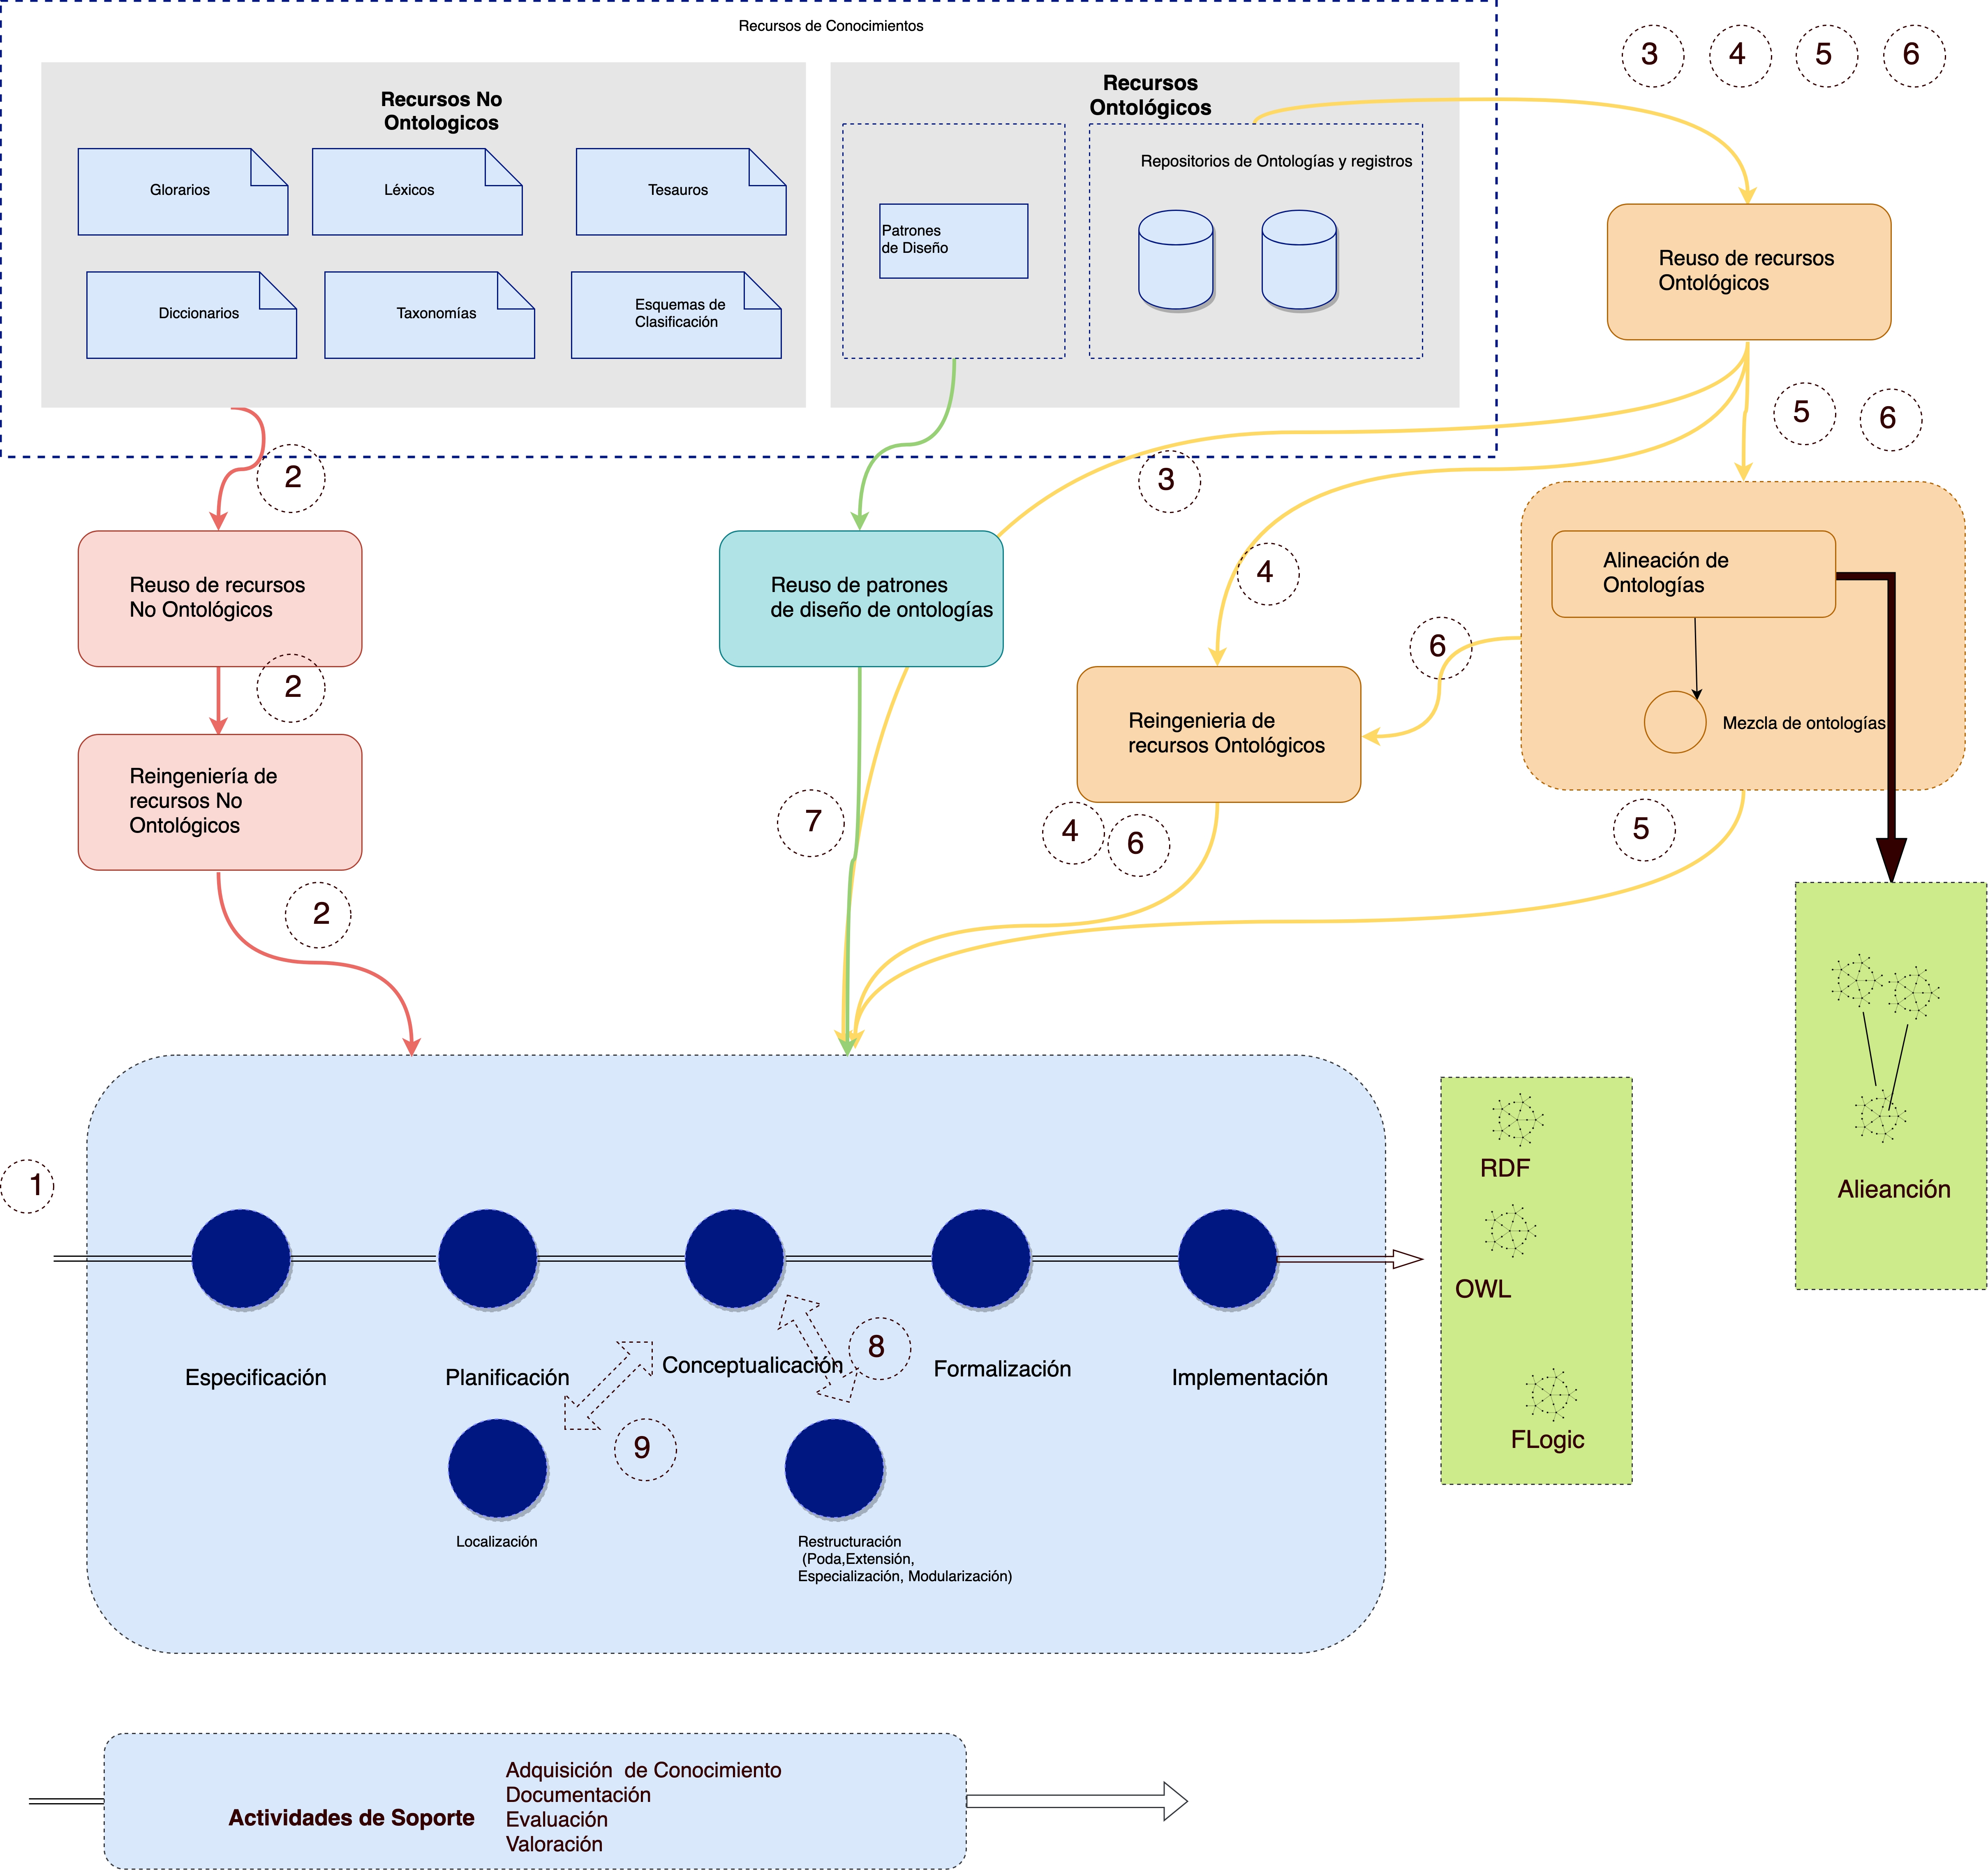
\includegraphics[width=150mm]{figuras/Diagramas-NeonProcess}
    \caption{Ciclo de vida de NeOn}
    \label{img:neon ciclo de vida}
    \end{figure}

El proceso de desarrollo de una ontología es definido como un proceso en el cual las necesidades de un usuario son convertidas a una ontología. Esto significa que el proceso se puede ver como un caso específico del proceso de desarrollo de software.	
El ciclo de vida es un modelo que describe cómo construir y mantener un proyecto ontológico, osea cómo ordenar los procesos y actividades en fases. Se pueden tener dos tipos de ciclo de vida que son:

\begin{itemize}
    \item Modelo de ciclo de vida de tipo cascada: En este modelo cada fase debe ser culminada antes de avanzar a la siguiente, no se permite retroceso excepto en el caso de la fase de mantenimiento. Este modelo es ideal cuando el tiempo de desarrollo es acotado y el dominio de conocimiento a modelar es bien conocido.
    \item Modelo de ciclo de vida de tipo iterativo-incremental: cada iteración es similar al modelo de cascada. Es ideal cual existe mucha incertidumbre acerca del alcance de la ontología a modelar.
\end{itemize}

A continuación exponemos los 5 modelos de ciclo de vida:	

\begin{description}
    \item[Modelo cascada de 4 fases.] Representa las etapas de una red de ontologías, comenzando con la Fase de Iniciación y yendo a través de la Fase de Diseño y Fase de Implementación hasta la Fase de Mantenimiento.
    \item[Modelo cascada de 5 fases.] Extiende el modelo de 4 fases con el reuso de recursos  ontológicos tales como son.
    \item[Modelo cascada de 5 fases + mezcla.] Es un caso especial del modelo de 5 fases. Incluye la Fase de Mezcla para obtener un nuevo recurso ontológico a partir de dos o más recursos ontológicos previamente seleccionados en la Fase de Reuso.
    \item[Modelo cascada de 6 fases.] Extiende el modelo de 5 fases con la Fase de Reingeniería. Permite la reingeniería de recursos de conocimiento (ontológicos y no-ontológicos). Puede ocurrir que algunos recursos de conocimiento son transformados en ontologías en la Fase de Reingeniería.
    \item[Modelo cascada de 6 fases + Mezcla.] Extiende el modelo de 6 fases incluyendo la Fase de Mezcla luego de la Fase de Reuso.
\end{description}

Los escenarios están ligados a un modelo dentro del ciclo de vida, como se muestra en la Tabla \ref{escenarios vs modelo}.

\begin{table}[tbp]
\centering
\caption{Escenarios vs Modelo}
\label{escenarios vs modelo}
\resizebox{15cm}{!} {
\begin{tabular}{|l|C|c|c|c|c|}
\hline
 & \multicolumn{1}{|m{2cm}|}{Modelo de 4-fases} & \multicolumn{1}{|m{2cm}|}{Modelo de 5-fases} & \multicolumn{1}{|m{2cm}|}{Modelo de 5-fases + mezcla} & \multicolumn{1}{|m{2cm}|}{Modelo de 6-fases} & \multicolumn{1}{|m{2cm}|}{Modelo de 6-fases + mezcla} \\ \hline
 Escenario 1 & x & & & & \\ \hline
 Escenario 2 & \multicolumn{1}{|m{2cm}|}{} & \multicolumn{1}{|m{2cm}|}{} & \multicolumn{1}{|m{2cm}|}{} & \multicolumn{1}{|m{2cm}|}{x} & \multicolumn{1}{|m{2cm}|}{} \\ \hline
 Escenario 3 & \multicolumn{1}{|m{2cm}|}{} & \multicolumn{1}{|m{2cm}|}{x} & \multicolumn{1}{|m{2cm}|}{} & \multicolumn{1}{|m{2cm}|}{} & \multicolumn{1}{|m{2cm}|}{} \\ \hline
 Escenario 4 & \multicolumn{1}{|m{2cm}|}{} & \multicolumn{1}{|m{2cm}|}{} & \multicolumn{1}{|m{2cm}|}{} & \multicolumn{1}{|m{2cm}|}{x} & \multicolumn{1}{|m{2cm}|}{} \\ \hline
 Escenario 5 & \multicolumn{1}{|m{2cm}|}{} & \multicolumn{1}{|m{2cm}|}{} & \multicolumn{1}{|m{2cm}|}{x} & \multicolumn{1}{|m{2cm}|}{} & \multicolumn{1}{|m{2cm}|}{} \\ \hline
 Escenario 6 & \multicolumn{1}{|m{2cm}|}{} & \multicolumn{1}{|m{2cm}|}{} & \multicolumn{1}{|m{2cm}|}{} & \multicolumn{1}{|m{2cm}|}{} & \multicolumn{1}{|m{2cm}|}{x} \\ \hline
 Escenario 7 & \multicolumn{1}{|m{2cm}|}{} & \multicolumn{1}{|m{2cm}|}{} & \multicolumn{1}{|m{2cm}|}{} & \multicolumn{1}{|m{2cm}|}{x} & \multicolumn{1}{|m{2cm}|}{} \\ \hline
 Escenario 8 & \multicolumn{1}{|m{2cm}|}{} & \multicolumn{1}{|m{2cm}|}{} & \multicolumn{1}{|m{2cm}|}{x} & \multicolumn{1}{|m{2cm}|}{} & \multicolumn{1}{|m{2cm}|}{} \\ \hline
 Escenario 9 & \multicolumn{1}{|m{2cm}|}{} & \multicolumn{1}{|m{2cm}|}{} & \multicolumn{1}{|m{2cm}|}{x} & \multicolumn{1}{|m{2cm}|}{} & \multicolumn{1}{|m{2cm}|}{} \\ \hline
\end{tabular}
}
\end{table}



\section{Herramientas tecnológicas}
En esta sección presentaremos las herramientas tecnológicas estudiadas para el desarrollo de este trabajo. Se presenta un editor de ontologías llamado Protégé (ver \ref{subsection:protege}), un visualizador de ontologías en formato de grafo llamado VOWL (ver \ref{subsection:vowl}), un framework para la manipulación de datos en RDF, RDFS y OWL llamado Apache Jena (ver \ref{subsection:jena}) y una herramienta para realizar consultas SPARQL llamado Apache Jena Fuseki (ver \ref{subsection:fuseki}) .
\subsection{Protégé}
\label{subsection:protege}
Protégé es una herramienta de código libre para desarrolladores de ontologías y permite crear sistemas de base de conocimientos. El editor consiste en una interfaz gráfica de usuario donde podemos crear y editar clases, instancias, propiedades y restricciones. Nos permite guardar la ontología en varios formatos como XML, RDF, TTL y OWL. En la Figura \ref{img:protege} se muestra una captura de pantalla de la herramienta.

\begin{figure}[h!]
    \centering
    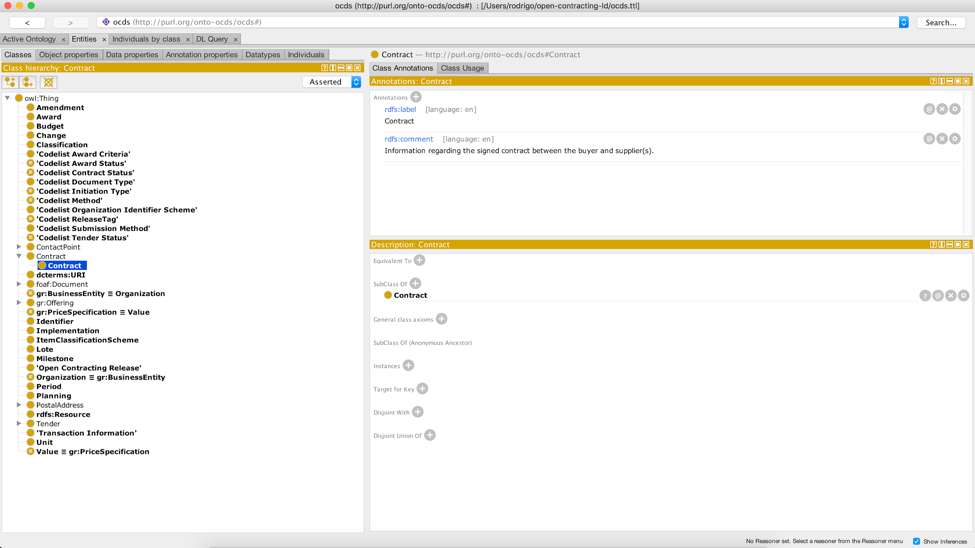
\includegraphics[width=150mm]{figuras/protege}
    \caption{Herramienta de Desarrollo de Ontologías: Protégé}
    \label{img:protege}
    \end{figure}

\subsection{Visual Notation for OWL}
\label{subsection:vowl}
Además se utilizó una herramienta de visualización gráfica de ontologías llamada \textit{Visual Notation for OWL} (VOWL) en su versión Web para visualizar de forma gráfica las ontologías estudiadas, en la Figura \ref{img:webvowl} se presenta una captura de pantalla de la herramienta utilizando como ejemplo una ontología llamada FOAF.

\begin{figure}[h!]
    \centering
    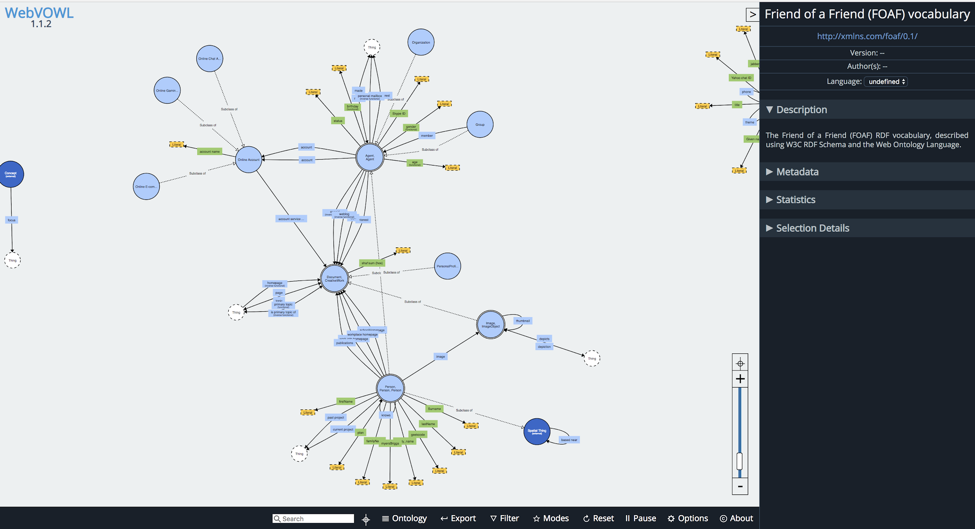
\includegraphics[width=150mm]{figuras/webvowl}
    \caption{Herramienta de Visualización de Ontologías: WebVOWL}
    \label{img:webvowl}
    \end{figure}
    

\subsection{Apache Jena}
\label{subsection:jena}
Jena es un \textit{Framework} implementado en JAVA para construir aplicaciones de la Web Semántica. Provee una librería para la manipulación de datos en RDF, RDFS, RDFa, OWL y SPARQL, y está alineada con las recomendaciones de la W3C. Jena incluye un motor de inferencias basado en reglas para realizar los razonamientos basados en OWL y RDFS, además de una variedad de estrategias para el almacenamiento de triplas RDF en memoria y en disco.

\subsection{Consulta de datos con SPARQL}
\label{subsection:fuseki}
Para consultar triplas basadas en RDF han surgido varios lenguajes de consulta, pero SPARQL es el más ampliamente utilizado y fue estandarizado por la W3C \cite{SPARQLDpoc:online}. Una consulta SPARQL es formulada usando patrones de grafos que pueden ser combinados con operaciones algebraicas como unión, opcional, filtro, etc. El resultado de la consulta es una lista de relaciones que pueden estar expresadas en tablas o en RDF.

A forma de explicar la semántica y sintaxis completa de este lenguaje, en el Cuadro \ref{lst:consulta-sparql} se muestra en un ejemplo la utilización del lenguaje realizando una consulta básica a la base de datos de DBPEDIA \cite{DBpedia:online} donde se listaron los nombres, fechas de nacimiento, fallecimiento y las URIs de personas nacidas en Paraguay antes de 1900, ordenadas por nombre.\hfill \break

\lstset{
    language=SPARQL
}
\noindent\begin{minipage}{\textwidth}
\begin{lstlisting}[captionpos=b, caption=Ejemplo de consulta SPARQL, label=lst:consulta-sparql,  numbers=left,  numberstyle=\tiny\color{mygray},
    basicstyle=\footnotesize\ttfamily,frame=single]
PREFIX dbo: <http://dbpedia.org/ontology/>
PREFIX xsd: <http://www.w3.org/2001/XMLSchema#>
PREFIX foaf: <http://xmlns.com/foaf/0.1/>
PREFIX : <http://dbpedia.org/resource/>

SELECT ?name ?birth ?death ?person WHERE { 

?person dbo:birthPlace :Paraguay . 
?person dbo:birthDate ?birth . 
?person foaf:name ?name . 
?person dbo:deathDate ?death . 
FILTER (?birth < "1900-01-01"^^xsd:date) . 

}
ORDER BY ?name
 
\end{lstlisting}
\end{minipage}

En las líneas 1 al 4 se pueden ver los prefijos de las ontologías utilizadas en la consulta, luego se presentan las triplas que componen las restricciones de la consulta. Está fuera del alcance de este documento la explicación detallada de la sintaxis de SPARQL.

Apache Jena Fuseki es un Servidor o Punto SPARQL que además provee un motor de inferencias. Se ejecuta como una aplicación web Java (archivo WAR). Provee el protocolo de consulta y actualización SPARQL 1.1 así como también el protocolo de \textit{SPARQL Graph Store}.

\section{Discusión del Capítulo}
En este capítulo se vieron los conceptos sobre Linked Open Data, Web Semántica y el rol de las ontologías en la misma. Además se dio una introducción a RDF, RDFS y OWL que son formas de representación de ontologías y datos en la Web Semántica. Para poder realizar consultas a las base de datos en RDF se dió una breve introducción del lenguaje SPARQL.

Se revisaron las metodologías más utilizadas para el desarrollo de una ontología para luego hacer una comparación de cada una de ellas presentadas en la Tabla \ref{tab:comparacion}. En cuanto a la madurez y completitud de cada una podemos decir que la metodología NeOn es la que mejor se posiciona, ya que la misma está basada en metodologías de desarrollo de software y metodologías de ingeniería de conocimiento. Además contempla escenarios de reuso de recursos ontológicos y no-ontológicos, los cuales serán necesarios para el desarrollo de este trabajo. Por este motivo se eligió NeOn como metodología base para el desarrollo de la ontología.

Además presentamos las herramientas tecnológicas utilizadas para el desarrollo de ontologías y posterior consulta a través de un servidor de consultas llamado Punto SPARQL.

En el siguiente capítulo comenzaremos con el desarrollo de la ontología utilizando la metodología NeOn.

